% A sample homework in LaTeX.
\documentclass[11pt]{article} % This marks the beginning of the LaTeX file.  Everything
                              % between here and \begin{document} is the preamble.
                              % The preamble contains global formatting commands and
                              % does not actually produce any text on the page.
\usepackage{graphicx}         % package for including and manipulating images
\usepackage{amsmath}          % extra math features
\usepackage{amssymb}          % extra math symbols
\usepackage{latexsym}         % extra symbols

% The following commands define the margins on the page.
% See page 182 in the Lamport book for the best explanation of these.
\topmargin      -0.25in
\headheight     0.0in
\headsep        0.0in
\textheight     9.5in
\textwidth      6.5in
\footskip       0.25in
\oddsidemargin  0.0in
\evensidemargin 0.0in

\parindent=0.0in       % don't indent paragraphs at all
\parskip 6pt           % skip 6 points between paragraphs

\begin{document}     % This marks the beginning of the document itself.
\begin{raggedleft}   % The raggedleft environment right justifies text.
Emma Steinman\\      % The \\ is the line break command.
CS 234 Homework 3\\
\today\\
\end{raggedleft}

% The enumerate environment produces a numbered list, perfect for homework.  
% Each item in the list is preceded by an \item.
\begin{enumerate}
\item[1.] Write a state trajectory for each of the three strings, 0001, 01101, and 00001101, along with determining accept/reject.
\begin{eqnarray*}0001: & q_0 \overset{0}{\rightarrow} q_0 \overset{0}{\rightarrow} q_0 \overset{0}{\rightarrow} q_0 \overset{1}{\rightarrow} q_1 & \textrm{accept} \\ 01101: & q_0 \overset{0}{\rightarrow} q_0 \overset{1}{\righarrow} q_1 \overset{1}{\rightarrow} q_2 \overset{0}{\rightarrow} q_2 \overset{1}{\rightarrow} q_1 & \textrm{accept} \\ 00001101: & q_0 \overset{0}{\rightarrow} q_0 \overset{0}{\rightarrow} q_0 \overset{0}{\rightarrow} q_0 \overset{0}{\rightarrow} q_0 \overset{1}{\rightarrow} q_1 \overset{1}{\rightarrow} q_2 \overset{0}{\rightarrow} q_2 \overset{1}{\rightarrow} q_1 &\textrm{accept} \\
\end{eqnarray*}
\item[5b.] Draw a state transition graph and also give the formal set notation for\\ $L=\{ab^{4}wb^{2}:w\in \{a,b\}^{*}\}$.
\begin{eqnarray*} 
M= \{Q, \Sigma, \delta, q_0, F\} \\ Q = \{q_0, q_1, q_2, q_3, q_4, q_5, q_6, q_7\}\\ \Sigma = \{a,b\}\\
F = \{q_6\} \\ \delta = \begin{array}{c | c c} & a & b\\ \hline q_0 & q_1 & q_7 \\ q_1 & q_7 & q_2 \\ q_2 & q_7 & q_3 \\ q_3 & q_7 & q_4 \\ q_4 & q_5 & q_4 \\ q_5 & q_6 & q_7 \\ q_6 & q_6 & q_7 \\ q_7 & q_7 & q_7 \end{array}\\
\end{eqnarray*}
\begin{figure} [ht!]
    \centering
    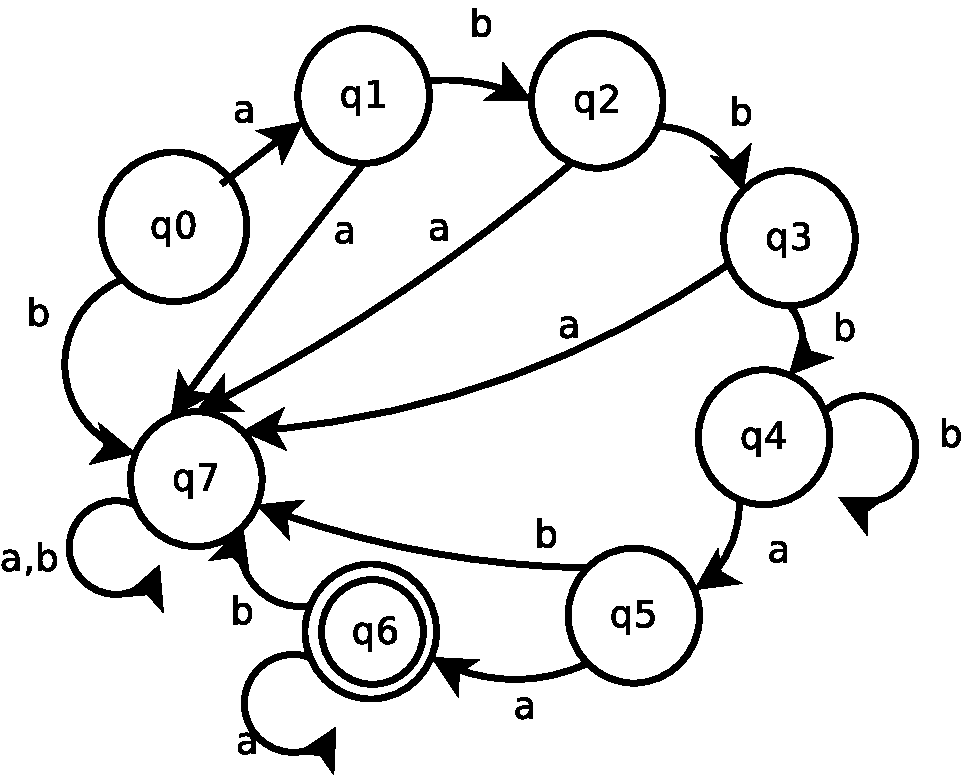
\includegraphics[width=2in]{5b.pdf}
\end{figure}


\item[5c.] Draw a state transition graph and also give the formal set notation for \\ 
$L=\{w_{1}abbw_{2} : w_{1}\in \{a,b\}^{*}, w_{2}\in \{a,b\}^{*}\}$.
\begin{eqnarray*}
M = \{Q, \Sigma, \delta, q_0, F\} \\ Q = \{q_0, q_1, q_2, q_3\} \\ \Sigma = \{a,b\} \\ F = \{q_3\} \\ 
\delta = \begin{array} {c | c c} & a & b\\ \hline q_0 & q_1 & q_0 \\ q_1 & q_1 & q_2 \\ q_2 & q_1 & q_3 \\ q_3 & q_3 & q_3 \\ \end{array}




\end{eqnarray*}
\item[6.] Draw a state transition graph and also give the formal set notation for \\ $L = \{w_{1}aw_{2} : |w_{1}| \geq 3, |w_{2}| \leq 4\}$. \\
\begin{eqnarray*}
M = \{Q, \Sigma, \delta, q_0, F\} \\ Q = \{q_0, q_1, q_2, q_3, q_4, q_5, q_6, q_7, q_8, q_9\}\\ \Sigma = \{a,b\} \\ F = \{q_4, q_5, q_6, q_7, q_8\} \\ \delta = \begin{array} {c | c c} & a & b \\ \hline q_0 & q_1 & q_1 \\ q_1 & q_2 & q_2 \\ q_2 & q_3 & q_3 \\ q_3 & q_4 & q_3 \\ q_4 & q_5 & q_5 \\ q_5 & q_6 & q_6 \\ q_6 & q_7 & q_7 \\ q_7 & q_8 & q_8 \\ q_8 & q_9 & q_9 \\ q_9 & q_9 & q_9 \\
\end{array}



\end{eqnarray*}
\item[13.] Draw a state transition graph and also give the formal set notation for \\ $L = \{vwv:v,w \in \{a,b\}^{*}, |v| = 3\}$ to show that it is regular. \\
\begin{eqnarray*}
M = \{Q, \Sigma, \delta, q_0, F\} \\ Q =\{q_0, q_1, q_2, q_3, q_4, q_5, q_6, q_7, q_8, q_9, q_{10}, q_{11}, q_{12}, q_{13}, q_{14}, q_{15}, q_{16},\\ q_{17}, q_{18}, q_{19}, q_{20}, q_{21}, q_{22}, q_{23}, q_{24}, q_{25}, q_{26}, q_{27}, q_{28}, q_{29},\\ q_{30}, q_{31}, q_{32}, q_{33}, q_{34}, q_{35}, q_{36}, q_{37}, q_{38}\} \\
\Sigma = \{a,b\} \\ F = \{q_{31}, q_{32}, q_{33}, q_{34}, q_{35}, q_{36}, q_{37}, q_{38}\} \\ 
\delta = \begin{array} {c | c c} &a & b\\ \hline q_0 & q_1 & q_2\\ q_1 & q_3 & q_4 \\ q_2 & q_5 & q_6\\ q_3 & q_7 & q_8\\ q_4 & q_9 & q_{10}\\ q_5 & q_{11} & q_{12}\\ q_6 & q_{13} & q_{14}\\ q_7 & q_{15} & q_7\\ q_8 & q_{16} & q_8\\ q_9 & q_{17} & q_9\\ q_{10} & q_{18} & q_{10}\\ q_{11} & q_{11} & q_{19}\\ q_{12} & q_{12} & q_{20}\\ q_{13} & q_{13} & q_{21}\\ q_{14} & q_{14} & q_{22}\\ q_{15} & q_{23} & q_7\\ q_{16} & q_{24} & q_8\\ q_{17} & q_{17} & q_{25}\\ q_{18} & q_{18} & q_{26}\\ q_{19} & q_{27} & q_{19}\\ q_{20} & q_{28} & q_{20}\\ q_{21} & q_{13} & q_{29}\\ q_{22} & q_{14} & q_{30}\\ q_{23} & q_{31} & q_7\\ q_{24} & q_{24} & q_{32}\\ q_{25} & q_{33} & q_9\\ q_{26} & q_8 & q_{34}\\ q_{27} & q_{35} & q_{19}\\ q_{28} & q_{12} & q_{36}\\ q_{29} & q_{37} & q_{29}\\ q_{30} & q_{14} & q_{38}\\ q_{31} & q_{31} & q_7\\ q_{32} & q_8 & q_8\\ q_{33} & q_9 & q_{25}\\ q_{34} & q_{18} & q_{10}\\ q_{35} & q_{11} & q_{19}\\ q_{36} & q_{28} & q_{20}\\ q_{37} & q_{13} & q_{13}\\ q_{38} & q_{14} & q_{38}\\\end{array}
\end{eqnarray*}






\end{enumerate}
\end{document}
 